\chapter{Análisis del sistema}
En este capítulo se presenta un análisis detallado del sistema a desarrollar,
desglosando las funcionalidades principales en epics y historias de usuario.
Este enfoque permite una visión estructurada del proyecto, facilitando su
planificación y desarrollo.

\section{Epics}
Los \textit{epics} representan las grandes áreas funcionales del proyecto.
Se han identificado las siguientes historias épicas:

\begin{enumerate}
    \item Infraestructura y despliegue
    \item Ingesta de datos
    \item Procesamiento y almacenamiento de datos
    \item Visualización y análisis
\end{enumerate}

Cada uno de estos epics engloba un conjunto de funcionalidades relacionadas
que, en conjunto, conforman el proyecto planteado.

\newpage{}
\section{Historias de usuario}
Las historias de usuario describen las funcionalidades específicas desde la
perspectiva del usuario final. A continuación, se detallan las historias de
usuario para cada epic:

\subsection{Epic 1: Infraestructura y despliegue}
Este epic se centra en la creación y gestión de la infraestructura necesaria
para el sistema.

\begin{itemize}
    \item \textbf{HU1.1:} Como desarrollador de Okticket, quiero poder
    desplegar un prototipo del sistema en mi entorno local para facilitar el
    desarrollo y las pruebas iniciales.

    \item \textbf{HU1.2:} Como desarrollador de Okticket, quiero que la
    arquitectura se despliegue y orqueste de manera automática en la nube para
    facilitar la gestión y el paso a producción del sistema.

    \item \textbf{HU1.3:} Como administrador del sistema, quiero que la
    infraestructura sea capaz de escalar automáticamente en función de la
    demanda para optimizar el rendimiento y los costos.
	\end{itemize}

\subsection{Epic 2: Ingesta de datos}
La ingesta de datos es fundamental para el funcionamiento del sistema,
abarcando diversas fuentes de información.

\begin{itemize}
    \item \textbf{HU2.1:} Como desarrollador de Okticket, quiero que se
    ingesten de manera automática datos de la base de datos interna de MongoDB
    para centralizar la información.
    \item \textbf{HU2.2:} Como desarrollador de Okticket, quiero que se
    ingesten de manera automática datos de la base de datos interna de MySQL
    para tener una visión completa de los datos.
    \item \textbf{HU2.3:} Como desarrollador de Okticket, quiero que se
    ingesten de manera automática logs de balanceador de AWS para monitorear
    el rendimiento de la infraestructura.
    \item \textbf{HU2.4:} Como desarrollador de Okticket, quiero poder ingestar
    datos de APIs externas a la empresa para enriquecer nuestros análisis.
    \item \textbf{HU2.5:} Como desarrollador de Okticket, quiero poder ingestar
    información de páginas web externas (scraping) para obtener datos
    adicionales relevantes.
\end{itemize}

\newpage{}
\subsection{Epic 3: Procesamiento y almacenamiento de datos}
Este epic se enfoca en la manipulación y organización eficiente de los datos
ingresados.

\begin{itemize}
    \item \textbf{HU3.1:} Como desarrollador de Okticket, quiero que los datos
    se limpien de manera automática para garantizar la calidad de la
    información.
    \item \textbf{HU3.2:} Como desarrollador de Okticket, quiero que los datos
    contengan metadatos que faciliten su filtrado o búsqueda para mejorar la
    eficiencia en el análisis.
\end{itemize}

\subsection{Epic 4: Visualización y análisis}
La visualización y análisis de datos es crucial para extraer valor de la
información recopilada.

\begin{itemize}
    \item \textbf{HU4.1:} Como trabajador de Okticket, quiero poder ver y
    consultar datos internos de la empresa para tomar decisiones informadas.
    \item \textbf{HU4.2:} Como desarrollador de Okticket, quiero poder ver el
    estado general de la infraestructura para monitorear su salud y rendimiento.
    \item \textbf{HU4.3:} Como trabajador de Okticket, quiero poder ver y
    consultar datos de empresas cliente para ofrecer un mejor servicio y
    soporte.
    \item \textbf{HU4.4:} Como gestor de una empresa cliente, quiero poder ver
    información relevante sobre mi empresa que recoja Okticket para optimizar
    mis procesos y tomar decisiones estratégicas.
\end{itemize}


\newpage{}
\section{Story Mapping}
El Story Mapping proporciona una visión de cómo las historias de usuario se
traducen en tareas concretas de desarrollo. Esta estrategia permite una
planificación más precisa y un seguimiento efectivo del progreso del proyecto.

\begin{figure}[h]
	\centering
	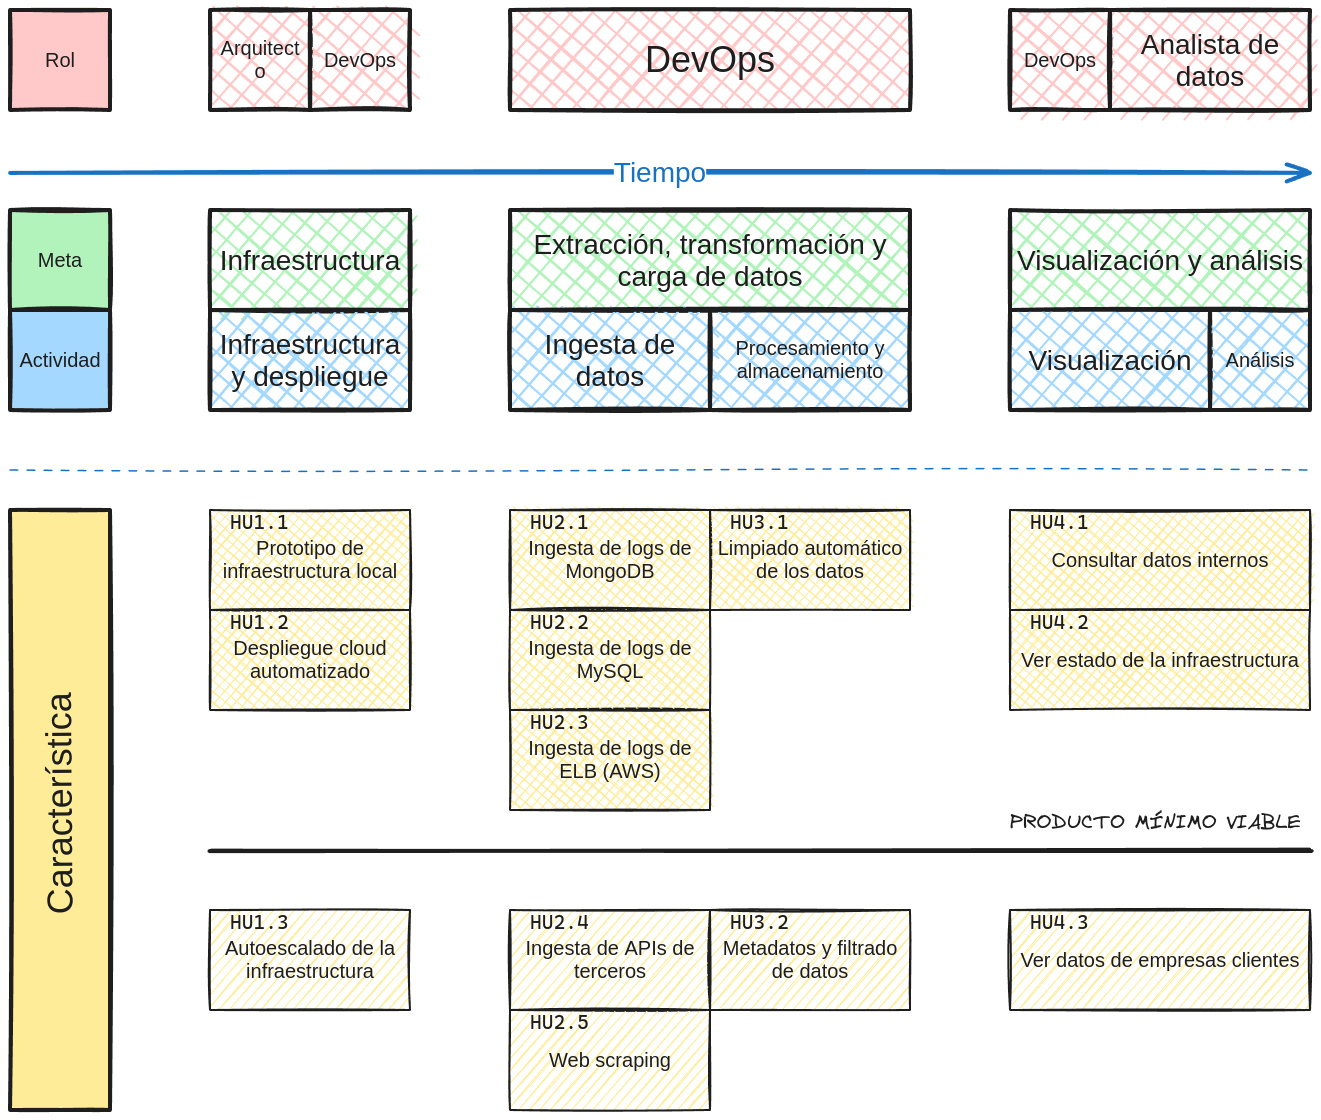
\includegraphics[width=\textwidth]{storymapping.png}
	\caption{Diagrama \textit{Story Mapping} del proyecto}
	\label{fig:story_mapping}
\end{figure}

El diagrama anterior muestra cómo las historias de usuario se organizan en
epics y se desglosan en tareas específicas. Esta representación visual ayuda a
comprender la estructura del proyecto y las dependencias entre las diferentes
historias y tareas.

Este \textit{story mapping} establece una hoja de ruta clara para el desarrollo
del proyecto, asegurando que todas las historias de usuario se aborden de manera
sistemática y eficiente.
